\documentclass[11pt,a4paper]{report}
\usepackage[utf8]{inputenc}
\usepackage[english]{babel}
\usepackage{amsmath}
\usepackage{hyperref}
\usepackage{breakurl}
\usepackage{amsfonts}
\usepackage{amssymb}
\usepackage{graphicx}
\begin{document}
%\maketitle
%Documentation for the car project
\section*{Embedded systems - Car project}
Johanna Vesterinen, Matthew Casserly, Carolina Lindqvist\\

\section*{Description}
The main schema for the car project can be seen in Fig. 1 \ref{car}.

\begin{figure}[h!]
\label{car}
\centering
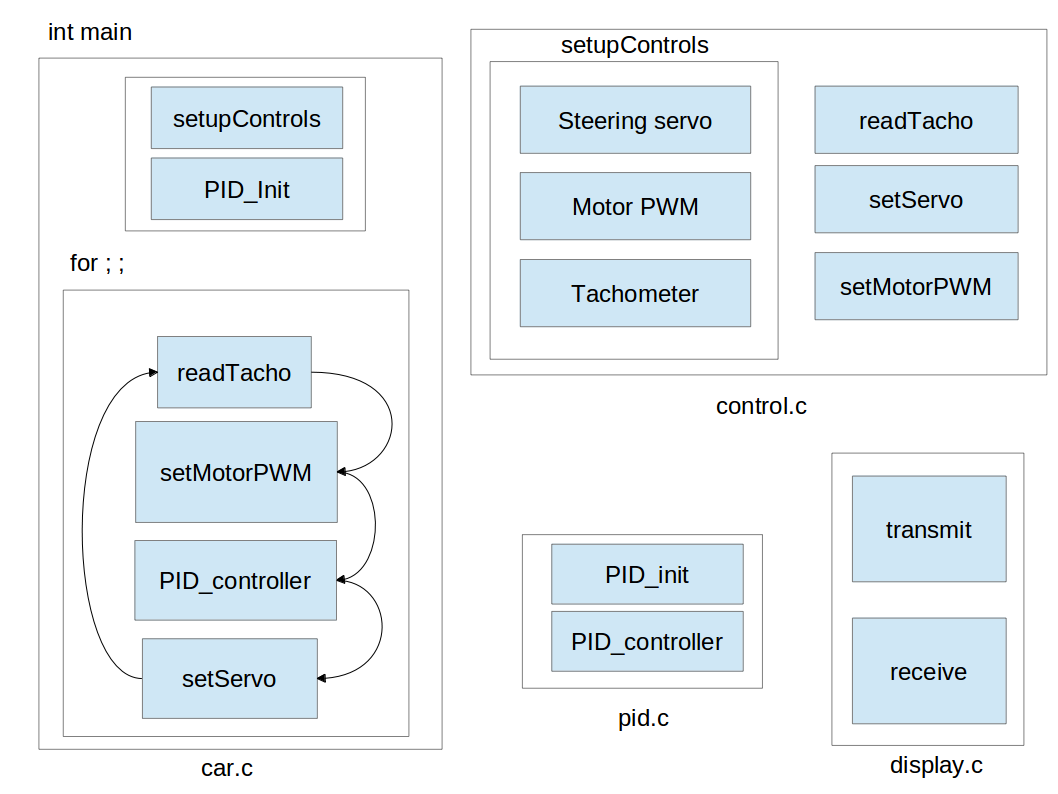
\includegraphics[scale=0.5]{car-schema.png}
\caption{Car project plan}
\end{figure}

\section*{Chosen settings}
The steering servo uses the Fast PWM mode with the prescaler value 8. It uses the set at bottom and "clear at match" settings. 
The motor PWM has the prescaler 1. Tachometer reading is done by an interrupt that regulates the motor PWM based on the readouts. The timer interrupt uses a \/64 prescaler. All prescaler values were chosen based on how well they fit with the 16 MHz clock, e.g. in order to regulate how often the tachometer readings updates (corrects) the speed.

\section*{Files}
\subsubsection*{car.*}
The car.c file contains the main for-loop that reads the steering sensors and adjusts the steering according to the sensor readings. A "start" button logic is also included, the for-loop starts executing as the black button is pressed.

\subsubsection*{control.*}
The control.* files contain the logic for regulating the speed and adjusting the direction the car travels in. The AVR chip configuration commands are also included (interrupts, timers, PWM, USART...) in the setupControls function. All eight sensors are read by the readSensors function. The functionality for setting the speed and reading the tachometer is included here. Speed is adjusted by the TIMER3\_COMPA\_vect interrupt.

\subsubsection*{display.*}
These files contain the control logic for the display. Input can be sent and received. It is based on the USART functionality from the AVR standard io library.

\end{document}
